\subsection{分次环上的整元}

本节考虑的分次都是 Z 型的；若 A 是分次环且 \(i \in Z\) ，则 \(A_{i}\) 表示环 A 的次数为 i 的齐次元组成的集。

设 A 是分次环，B 是分次 A-代数。设 x 是 B 的在 A 上整的齐次元；则存在关系式

\[
x ^ {n} + a _ {1} x ^ {n - 1} + \dots + a _ {n} = 0 \quad \text { where } \quad a _ {i} \in A \quad \text { for } \quad 1 \leqslant i \leqslant n.\tag{3}
\]

设 \(m = \deg(x)\) ，并设 \(a_i'\) 是 \(mi\) 次齐次分量（\(a_i\) 的）（ \(1 \leqslant i \leqslant n\) ）；则显然

\[
x ^ {n} + a _ {1} ^ {\prime} x ^ {n - 1} + \dots + a _ {n} ^ {\prime} = 0\tag{4}
\]

换言之，x 满足一个系数为齐次元的整依赖方程。

用 \(\mathbf{A}[\mathbf{X},\mathbf{X}^{-1}]\) 表示分式环 \(\mathbf{S}^{-1}\mathbf{A}[\mathbf{X}]\) ，即单未定元多项式环 \(\mathbf{A}[\mathbf{X}]\) 的分式环，其中 \(\mathbf{S}\) 是 \(\mathbf{A}[\mathbf{X}]\) 中由方幂 \(\mathbf{X}^n\) （\(\mathbf{X}\) 的方幂， \(n\geqslant 0\) ）组成的乘性子集；由于 \(\mathbf{X}\) 不是 \(\mathbf{A}[\mathbf{X}]\) 中的零因子，立即可见诸 \(\mathbf{X}^i\)（ \(i\in \mathbf{Z}\) ）构成 \(\mathbf{A}\) 上 A-模 \(\mathbf{A}[\mathbf{X},\mathbf{X}^{-1}]\) 的一组基。对每个元素 \(a\in \mathbf{A}\) ，其齐次分量为 \(a_{i}\)（ \(i\in \mathbf{Z}\) ），我们记

\iffalse
\begin{description}
\tightlist
\item[\$\$]
j \_ \{\mathbf {A}\} (a) = \sum\_ \{i \in \mathbf {Z}\} a \_ \{i\} \mathbf {X} \^{} \{i\} \in \mathrm{A} {[} \mathbf {X}, \mathbf {X} \^{} \{- 1\} {]}\tag{5} \$\$
\end{description}
\fi

\[
:j_{A}(a) = \sum_{i \in \mathbf{Z}} a_{i} \mathbf{X}^{i} \in \mathbf{A}[\mathbf{X},\mathbf{X}^{-1}]\tag{5}
\]

立即可见 \(j_{A}: A \to A[X, X^{-1}]\) 是单的环同态。

命题 20. 设 \(\mathbf{A} = \bigoplus_{i\in \mathbf{Z}}\mathbf{A}_i\) 是分次环，\(\mathbf{B}\) 是（交换）分次 A-代数。集 \(\mathbf{A}'\) 由 \(\mathbf{B}\) 中在 \(\mathbf{A}\) 上整的元素组成，它是 \(\mathbf{B}\) 的分次子代数。若 \(\mathbf{A}_i = 0\) （\(i < 0\)）且 \(\mathbf{B}\) 是约化环，则 \(\mathbf{A}_i' = 0\) （\(i < 0\)）。

若 \(\mathbf{A}_i = 0\) （\(i < 0\)）且 \(\mathbf{B}\) 是约化环，则 \(\mathbf{A}_i' = 0\) （\(i < 0\)）。图

\pandocbounded{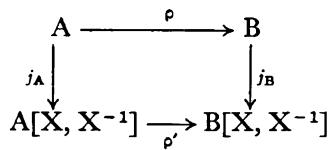
\includegraphics[keepaspectratio]{images/part002_18d5f867.jpg}}

（其中 \(\rho\) 是定义 B 上 A-代数结构的同态，\(\rho'\) 是由它典范导出的同态）是交换的，这由定义 (5) 立即验证。设 \(x\) 是 B 中在 A 上整的元素；则 \(j_{\mathrm{B}}(x)\) 在 \(\mathbf{A}[\mathbf{X}, \mathbf{X}^{-1}]\) 上是整的（第 1 节，命题 2），因此由第 5 节命题 16 可知，存在整数 \(m > 0\) 使得 \(\mathbf{X}^m j_{\mathrm{B}}(x)\) 是 \(\mathbf{B}[\mathbf{X}]\) 中在 \(\mathbf{A}[\mathbf{X}]\) 上整的元素。再由第 3 节命题 12 推出多项式 \(\mathbf{X}^m j_{\mathrm{B}}(x)\) 的系数在 A 上是整的；由于这些系数按定义就是 \(x\) 的齐次分量，可见它们都在 A 上是整的，这就证明了 \(\mathbf{A}'\) 是 B 的分次子代数。

现在设 \(x \in \mathbf{A}_i'\) ，其中 \(i < 0\) ；本节开头的注表明 \(x\) 满足形如 (4) 的方程，其中 \(a_k' \in \mathbf{A}_{ki}\) （\(1 \leqslant k \leqslant n\)）。若 \(\mathbf{A}_j = 0\) （\(j < 0\)），则 \(x^n = 0\) ；又若 \(B\) 是约化环，则可断定 \(x = 0\) ，从而在此情形 \(\mathbf{A}_i' = 0\) （对所有 \(i < 0\)）。

回忆（第 II 章，§ 2，第 9 节）：若 \(\mathbf{A} = \bigoplus_{i\in \mathbf{Z}}\mathbf{A}_i\) 是分次环，S 是由齐次元组成的 A 的乘性子集，则在 \(\mathrm{S}^{-1}\mathrm{A}\) 上可定义一个分次环结构，只需把集 \((\mathrm{S}^{-1}\mathrm{A})_i\) （\(i\) 次齐次元组成的集）取作形如 \(a / s\) 的元素组成的集，其中 \(a\in \mathbf{A}\) 与 \(s\in \mathbf{S}\) 是齐次的，且 \(\deg (a) - \deg (s) = i\) 。

引理 4. 设 \(\mathbf{A} = \bigoplus_{i\in \mathbf{Z}}\mathbf{A}_i\) 是分次整环，S 是 A 的 \(\neq 0\) 齐次元组成的集。

\begin{enumerate}
\def\labelenumi{(\roman{enumi})}
\item
  每个 \(\neq 0\) 的齐次元（\(\mathbf{S}^{-1}\mathbf{A}\) 中的）都是可逆的，环 \(\mathbf{K}_0 = (\mathbf{S}^{-1}\mathbf{A})_0\) 是域，且诸 \(i\in \mathbf{Z}\) 中使 \((\mathrm{S}^{-1}\mathrm{A})_i\neq 0\) 者组成的集是子群 \(q\mathbf{Z}\) ——\(\mathbf{Z}\) 的子群（其中 \(q\geqslant 0\) ）。
\item
  假设 \(q \geqslant 1\) ，并设 \(t\) 是 \((\mathbf{S}^{-1}\mathbf{A})_q\) 的非零元素。则 \(\mathbf{K}_0\) -同态 \(f\) （它把多项式环 \(\mathbf{K}_0[\mathbf{X}]\) 映到 \(\mathbf{S}^{-1}\mathbf{A}\) ，把 \(\mathbf{X}\) 映到 \(t\) ）可扩张为 \(\mathbf{K}_0[\mathbf{X}, \mathbf{X}^{-1}]\) 到 \(\mathbf{S}^{-1}\mathbf{A}\) 上的同构，且 \(\mathbf{S}^{-1}\mathbf{A}\) 是整闭的。
\end{enumerate}

(i) 中的断言由诸定义及 A 是整环这一假设立即得出，因为若 \(a/s\) 与 \(a'/s'\) 是两个 \(\neq 0\) 齐次元，属于 \(\mathrm{S}^{-1}\mathrm{A}\) ，次数分别为 \(i\) 与 \(i'\) ，则 \(aa'/ss'\) 是 \(\neq 0\) 齐次元，且次数为 \(i+i'\) 。为证 (ii)，注意由于 \(t\) 在 \(\mathrm{S}^{-1}\mathrm{A}\) 中可逆，同态 \(f\) 以唯一方式扩张为同态 \(\bar{f}: \mathrm{K}_0[\mathrm{X}, \mathrm{X}^{-1}] \to \mathrm{S}^{-1}\mathrm{A}\) ，且必有 \(\bar{f}(\mathrm{X}^{-1}) = t^{-1}\) 。另一方面，由 \(q\) 的定义，每个 \(\neq 0\) 齐次元（\(\mathrm{S}^{-1}\mathrm{A}\) 中的）的次数都形如 \(qn\)（ \(n \in \mathbf{Z}\) ），从而可唯一地写成 \(\lambda t^n\) 的形式，其中 \(\lambda \in \mathrm{K}_0\) （因为 \(\mathrm{S}^{-1}\mathrm{A}\) 是整环）；因此 \(\bar{f}\) 是双射。最后，我们知道 \(\mathrm{K}_0[\mathrm{X}]\) 是整闭的（第 3 节，命题 10），从而 \(\mathrm{K}_0[\mathrm{X}, \mathrm{X}^{-1}]\) 也是整闭的（第 5 节，命题 16 的推论 1），这就完成了引理的证明。

命题 21. 设 \(\mathbf{A} = \bigoplus_{i\in \mathbf{Z}}\mathbf{A}_i\) 是分次整环，S 是 A 的 \(\neq 0\) 齐次元组成的集。则 A 的整闭包 \(\mathbf{A}'\) 是 \(\mathbf{S}^{-1}\mathbf{A}\) 的分次子环。若进一步 \(\mathbf{A}_i = 0\) （\(i < 0\)），则 \(\mathbf{A}_i' = 0\) （\(i < 0\)）。

若 \(A = A_{0}\) ，命题是平凡的。否则可应用引理 4；环 \(S^{-1}A\) 是整闭整环，因此 \(A' \subset S^{-1}A\) ；由于 \(S^{-1}A\) 是分次的，由命题 20，\(A'\) 也是分次的；后一断言同样由命题 20 得出。

推论 1. 在命题 21 的假设与记号下，若 \(\mathbf{S}^{-1}\mathbf{A}\) 中在 \(\mathbf{A}\) 上是整的每个齐次元都属于 \(\mathbf{A}\) ，则 \(\mathbf{A}\) 是整闭的。

则 \(\mathbf{A}_i' \subset \mathbf{A}\) 对所有 \(i \in \mathbf{Z}\) 成立，从而 \(\mathbf{A}' = \mathbf{A}\) 。

推论 2. 若 \(\mathbf{A} = \bigoplus_{i\in \mathbf{Z}}\mathbf{A}_i\) 是整闭的分次整环，则整环 \(\mathbf{A}_0\) 是整闭的。

\(\mathbf{K}_0\) （\(\mathbf{A}_0\) 的分式域，按命题 21 的记号）被等同于

\(S^{-1}A\) 的由 0 次齐次元组成的环的一个子环；因此，\(K_{0}\) 中在 \(A_{0}\) 上（更不必说在 A 上）是整的每个元素按假设都属于 \(A_{0}\) 。

推论 3. 设 \(\mathbf{A} = \bigoplus_{i\in \mathbf{Z}}\mathbf{A}_i\) 是整闭的分次整环。则对每个整数 \(d > 0\) ，环 \(\mathbf{A}^{(d)}\) （第 III 章，§1，第 3 节）是整闭整环。

设 U 是由 \(\neq0\) 齐次元（\(A^{(d)}\) 中的）组成的集，并设 x 是 \(U^{-1}A^{(d)}\) 的在 \(A^{(d)}\) 上因而在 A 上是整的齐次元；由于 \(x\in S^{-1}A\) ，按假设 x 属于 A；由于其次数被 d 整除，它属于 \(A^{(d)}\) ，于是由推论 1 即得 \(A^{(d)}\) 是整闭的。

